\documentclass[presentation]{beamer}
\usepackage[utf8]{inputenc}
\usepackage[T1]{fontenc}
\usepackage{fixltx2e}
\usepackage{graphicx}
\usepackage{longtable}
\usepackage{float}
\usepackage{wrapfig}
\usepackage{rotating}
\usepackage[normalem]{ulem}
\usepackage{amsmath}
\usepackage{textcomp}
\usepackage{marvosym}
\usepackage[integrals]{wasysym}
\usepackage{amssymb}
\usepackage{hyperref}
\tolerance=1000
\usepackage{minted}
\usepackage{amsmath}
\usepackage{tikz}
\usepgflibrary{shapes.geometric}
\usetikzlibrary{calc}
\usetikzlibrary{positioning}
\usetikzlibrary{intersections,decorations.pathreplacing,shapes,arrows}
\usetikzlibrary{plotmarks}
\usepackage{amsmath,amssymb}
\usepackage{mathtools}
\DeclareMathOperator{\tr}{tr}
\usepackage{pgfplots}
\institute{Departments of Computing and Mathematics, Imperial College London}
\renewcommand{\vec}{\mathbf}
\usetheme{IC}
\author{Lawrence Mitchell}
\date{1st July 2015}
\title{Geometric multigrid without the agonising pain}
\begin{document}

\maketitle

\begin{frame}
  \frametitle{Outline}
  \tableofcontents
\end{frame}

\section{Introduction}
\begin{frame}
  \frametitle{Why multigrid?}
  \begin{itemize}[<+->]
  \item Large problems need \emph{fast} and \emph{scalable} solvers
  \item Fast: $\mathcal{O}(N)$ work
  \item Scalable: $\mathcal{O}(\log P)$ communication depth
  \item Multilevel methods offer this
  \end{itemize}

  \begin{block}<2->{Fast}
    Want to achieve error $||u - u_h|| < \epsilon$ in $\mathcal{O}(N)$
    work.
  \end{block}

  \begin{block}<3->{Scalable}
    Local work needs to scale like $N/P$

    Fast parallel algorithms have $\mathcal{O}(\log P)$ critical paths
    (communication depth).  Need this for solver too.
  \end{block}
\end{frame}



\section{Multigrid primer}

\begin{frame}
  \frametitle{A sketch history}
  \begin{itemize}[<+->]
  \item[1964] Fedorenko: two-level method for Laplacian, analysed in
    1D
  \item[1970s] Explosion in development of rigourous analysis and
    multilevel methods.  Development of techniques for non-elliptic
    problems
  \item[1980s] Multigrid for EVERYTHING!
    \visible<+->{Two guides to multilevel methods: Brandt (1984),
    Hackbusch (1985), more applications.  Multilevel methods as
    asymptotic direct solvers}
  \item[1990s] MG for preconditioning Krylov (MG for everything is too
    hard if you're not Achi)
  \item[2000s] MG for $H(\text{div}/\text{curl})$
  \item[now] Multilevel solvers a fact of life in HPC
  \end{itemize}
\end{frame}


\begin{frame}
  \frametitle{How does it work?}
  \begin{block}{A prototype linear equation}
    \begin{equation*}
      A(x) = b
    \end{equation*}
    \begin{itemize}
    \item Current guess: $\hat{x}$, with error $e = x - \hat{x}$ and 
      $r = b - A(\hat{x})$
    \item Residual equation: $A(x) - A(\hat{x}) = A(e) = r$
    \end{itemize}
  \end{block}
  \begin{visibleenv}<2->
    \begin{block}{Solution plan on two grids}
      \begin{itemize}[<+(1)->]
      \item Obtain residual on \emph{fine} grid: $r_f$
      \item \emph{Restrict} to coarse grid:
        $r_c \leftarrow \mathcal{R}(r_f)$
      \item Solve residual equation for the coarse error:
        $e_c \leftarrow A_c^{-1} r_c$
      \item \emph{Prolong} to fine grid and update solution:
        $\hat{x} \leftarrow \hat{x} + \mathcal{P}(e_c)$
      \end{itemize}
    \end{block}
  \end{visibleenv}
\end{frame}

\begin{frame}
  \frametitle{Components of the multigrid cycle}

  \begin{block}<+->{Smoothing}
    \begin{itemize}
    \item No need to \emph{solve} on fine grid
    \item Just need to \emph{smooth} components of the error which cannot
      be represented on coarse grids
    \end{itemize}
  \end{block}
  \begin{block}<+->{Transfer operators}
    \begin{itemize}
    \item [$\mathcal{R}$] residual restriction (fine to coarse)
    \item [$\mathcal{P}$] correction prolongation (coarse to fine)
    \end{itemize}
  \end{block}
  \begin{block}<+->{Coarse solves}
    \begin{itemize}
    \item Computing $A_c^{-1}$ directly not feasible unless very small
    \item Instead, apply two-grid scheme recursively
    \end{itemize}
  \end{block}
\end{frame}

\begin{frame}
  \frametitle{It's all about smoothing}
  \begin{itemize}
  \item Coarse grid is coarser, so some fine grid error modes will
    \emph{alias}
  \item \emph{Smoothing} on fine grid to reduce high-frequency,
    aliasing, modes
  \item Restriction now only sees fine-grid ``smooth'' errors, but
    they look coarse, remove them
  \item Prolongation will ``de-alias'' coarse grid modes,
    reintroducing some high frequency error, need to smooth this out
    too
  \end{itemize}

  \begin{block}<2>{Some smoothers}
    \begin{itemize}
    \item[Elliptic] pointwise is good (SOR, Jacobi, Gauss-Seidel)
    \item[!Elliptic] Need to inspect problem (and literature!): line
      smoothing, local overlapping ASM (e.g. for $H(\text{div})$),
      point block Jacobi (Vanka-like for flows), etc...
    \end{itemize}
  \end{block}
\end{frame}

\begin{frame}
  \frametitle{Grid transfer}
  \begin{itemize}
  \item Embedded spaces: $V_c \subset V_f$
  \item<+->[Got] $\int_\Omega f v_f \mathrm{d}x$
  \item<+->[Want] $\int_\Omega f v_c \mathrm{d}x$
  \item<+-> But $v_c \in V_f$, so write $v_c$ as linear combination of
    ${\phi_f}$
  \item<+-> Prolongation is natural (embedding), gives $\mathcal{P} =
    \mathcal{R}^{T}$
  \item<.-> Other options available, but then MG application may not be
    symmetric
  \end{itemize}
\end{frame}

\begin{frame}
  \frametitle{The V cycle}
  \begin{columns}
    \begin{column}{0.7\textwidth}
      \begin{itemize}
      \item Presmooth:
        $\hat{x} \leftarrow \mathcal{S}_\text{pre}(\hat{x})$
      \item Restrict residual:
        $r_c \leftarrow \mathcal{R}(b - A(\hat{x}))$
      \item Recurse on $A_c(e_c) = r_c$
      \item Prolong error and update:
        $\hat{x} \leftarrow \hat{x} + \mathcal{P}(e_c)$
      \item Postsmooth:
        $\hat{x} \leftarrow \mathcal{S}_\text{post}(\hat{x})$
      \end{itemize}
    \end{column}
    \begin{column}{0.3\textwidth}
      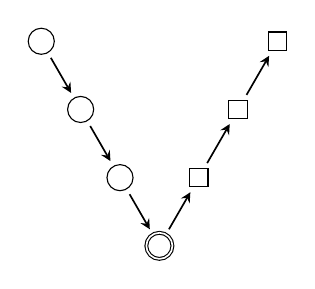
\begin{tikzpicture}[
        restrict/.style={-stealth, shorten <= 2pt, shorten >=
          2pt,semithick}, 
        prolong/.style={-stealth, shorten <=2pt, shorten >=2pt,
          semithick}, 
        presmooth/.style={draw, circle}, 
        coarse/.style={draw, circle, double},
        postsmooth/.style={draw}]
        \node[presmooth] (A) at (0,0) {};
        \node[presmooth] (B) at ($(A) + (-60:1)$) {};
        \node[presmooth] (C) at ($(B) + (-60:1)$) {}; 
        \node[coarse] (D) at ($(C) + (-60:1)$) {}; 
        \node[postsmooth] (E) at ($(D) + (60:1)$) {}; 
        \node[postsmooth] (F) at ($(E) + (60:1)$) {}; 
        \node[postsmooth] (G) at ($(F) + (60:1)$) {};

        \draw[restrict] (A) -- (B);
        \draw[restrict] (B) -- (C);
        \draw[restrict] (C) -- (D);
        \draw[prolong] (D) -- (E);
        \draw[prolong] (E) -- (F);
        \draw[prolong] (F) -- (G);
      \end{tikzpicture}
    \end{column}
  \end{columns}
  \begin{block}<2>{Computational complexity}
    \begin{itemize}
    \item Coarse grids halve in size, $d$ grids
    \item Fixed number of smooths per level
    \item Can achieve discretisation error in $\mathcal{O}(\log N)$ cycles
    \end{itemize}
    \begin{equation*}
      \text{cost} = \mathcal{O}\left(N
        \sum_{i=0}^{d-1}\frac{1}{2^i}\right) + \text{coarse solve}
    \end{equation*}
  \end{block}
\end{frame}

\begin{frame}
  \frametitle{Other cycle types}
  \begin{block}<1| only@1>{W cycle}
    Discretisation error in $\mathcal{O}(\log N)$ cycles
    \begin{center}
      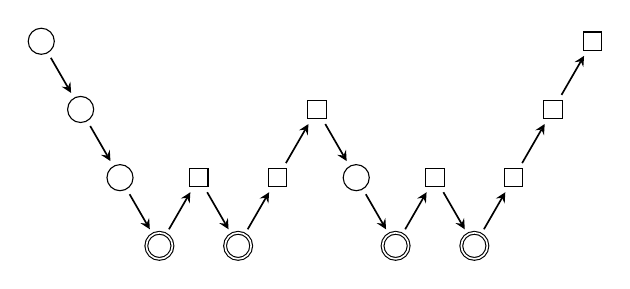
\begin{tikzpicture}[
        restrict/.style={-stealth, shorten <= 2pt, shorten >=
          2pt,semithick}, 
        prolong/.style={-stealth, shorten <=2pt, shorten >=2pt,
          semithick}, 
        presmooth/.style={draw, circle}, 
        coarse/.style={draw, circle, double},
        postsmooth/.style={draw}]
        \node[presmooth] (A) at (0,0) {};
        \node[presmooth] (B) at ($(A) + (-60:1)$) {};
        \node[presmooth] (C) at ($(B) + (-60:1)$) {}; 
        \node[coarse] (D) at ($(C) + (-60:1)$) {}; 
        \node[postsmooth] (E) at ($(D) + (60:1)$) {};
        \node[coarse] (F) at ($(E) + (-60:1)$) {}; 
        \node[postsmooth] (G) at ($(F) + (60:1)$) {};
        \node[postsmooth] (H) at ($(G) + (60:1)$) {};
        \node[presmooth] (I) at ($(H) + (-60:1)$) {};
        \node[coarse] (J) at ($(I) + (-60:1)$) {};
        \node[postsmooth] (K) at ($(J) + (60:1)$) {};
        \node[coarse] (L) at ($(K) + (-60:1)$) {};
        \node[postsmooth] (M) at ($(L) + (60:1)$) {};
        \node[postsmooth] (N) at ($(M) + (60:1)$) {};
        \node[postsmooth] (O) at ($(N) + (60:1)$) {};
        \draw[restrict] (A) -- (B);
        \draw[restrict] (B) -- (C);
        \draw[restrict] (C) -- (D);
        \draw[prolong] (D) -- (E);
        \draw[restrict] (E) -- (F);
        \draw[prolong] (F) -- (G);
        \draw[prolong] (G) -- (H);
        \draw[restrict] (H) -- (I);
        \draw[restrict] (I) -- (J);
        \draw[prolong] (J) -- (K);
        \draw[restrict] (K) -- (L);
        \draw[prolong] (L) -- (M);
        \draw[prolong] (M) -- (N);
        \draw[prolong] (N) -- (O);
      \end{tikzpicture}
    \end{center}
  \end{block}
  \begin{block}<2 | only@2>{F cycle (full multigrid)}
    Can achieve \emph{discretisation error} in $\mathcal{O}(1)$
    cycles, somewhat more forgiving than V- and W-cycles
    \begin{center}
      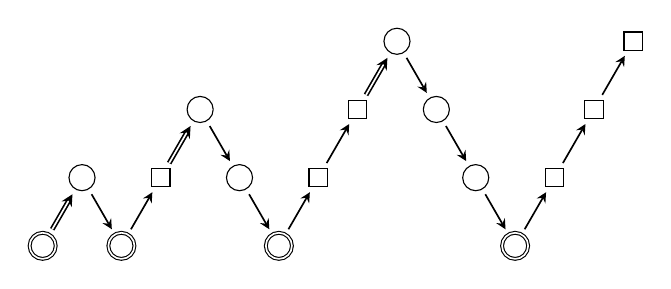
\begin{tikzpicture}[
        restrict/.style={-stealth, shorten <= 2pt, shorten >=
          2pt,semithick}, 
        prolong/.style={-stealth, shorten <=2pt, shorten >=2pt,
          semithick}, 
        presmooth/.style={draw, circle}, 
        coarse/.style={draw, circle, double},
        postsmooth/.style={draw},
        project/.style={-stealth, shorten <=2pt, shorten >=2pt,
          semithick, double}]
        \node[coarse] (A) at (0,0) {};
        \node[presmooth] (B) at ($(A) + (60:1)$) {};
        \draw[project] (A) -- (B); 
        \node[coarse] (C) at ($(B) + (-60:1)$) {};
        \draw[restrict] (B) -- (C);
        \node[postsmooth] (D) at ($(C) + (60:1)$) {};
        \draw[prolong] (C) -- (D);
        \node[presmooth] (E) at ($(D) + (60:1)$) {};
        \draw[project] (D) -- (E);
        \node[presmooth] (F) at ($(E) + (-60:1)$) {};
        \draw[restrict] (E) -- (F);
        \node[coarse] (G) at ($(F) + (-60:1)$) {};
        \draw[restrict] (F) -- (G);
        \node[postsmooth] (H) at ($(G) + (60:1)$) {};
        \draw[prolong] (G) -- (H);
        \node[postsmooth] (I) at ($(H) + (60:1)$) {};
        \draw[prolong] (H) -- (I);
        \node[presmooth] (J) at ($(I) + (60:1)$) {};
        \draw[project] (I) -- (J);

        \node[presmooth] (K) at ($(J) + (-60:1)$) {};
        \draw[restrict] (J) -- (K);
        \node[presmooth] (L) at ($(K) + (-60:1)$) {};
        \draw[restrict] (K) -- (L);
        \node[coarse] (M) at ($(L) + (-60:1)$) {};
        \draw[restrict] (L) -- (M);
        \node[postsmooth] (N) at ($(M) + (60:1)$) {};
        \draw[prolong] (M) -- (N);
        \node[postsmooth] (O) at ($(N) + (60:1)$) {};
        \draw[prolong] (N) -- (O);
        \node[postsmooth] (P) at ($(O) + (60:1)$) {};
        \draw[prolong] (O) -- (P);
      \end{tikzpicture}
    \end{center}
  \end{block}
\end{frame}

\begin{frame}
  \frametitle{Why not AMG?}
  \begin{itemize}
  \item For many problems, can \emph{just} use black or gray box AMG
  \item But, may not deal well with some anistropies
  \item Doesn't exploit structure in your problem
  \item Requires assembled operators (not great for the way modern
    hardware is going)
  \end{itemize}
\end{frame}

\begin{frame}
  \frametitle{Nonlinear multigrid}
  \begin{itemize}
  \item Recall residual equation $A(x) - A(\hat{x}) = r \neq A(e)$ if
    $A$ nonlinear
  \item Newton-MG: linearise and use MG for linear problem
  \item Full approximation scheme (FAS): apply MG directly
  \end{itemize}

  \begin{block}{FAS}
    \begin{itemize}
    \item Obtain guess on fine grid $\hat{x}_f$ with residual $r_f$
    \item Write $x_c = e_c + \hat{x}_c$
    \item Solve $A_c(x_c) = \mathcal{R}(r_f) + A_c(\mathbb{R}(\hat{x}_f))$
    \item Update fine solution: $\hat{x} \leftarrow \hat{x} +
      \mathcal{P}(x_c - \mathbb{R}(\hat{x}_f))$
    \item $\mathbb{R}$ ``state injection'' (need not be the same as
      residual restriction)
    \end{itemize}
  \end{block}
\end{frame}

\begin{frame}
  \frametitle{Pros and Cons}
    \begin{block}<1->{Newton-MG}
      \begin{itemize}
      \item Good theory on smoothers for linear problems
      \item Quadratic convergence near roots
      \item Requires \emph{global} linearisation
      \item High memory requirements, low flop rates (if using
        assembled matrices)
      \end{itemize}
    \end{block}
    \begin{block}<2->{FAS}
      \begin{itemize}
      \item Comparatively little theory
      \item Linear convergence near roots
      \item Requires only \emph{local} linearisation
      \item Lower memory requirements, potentially higher flop rates
      \end{itemize}
    \end{block}
\end{frame}

\section{Support in Firedrake}

\begin{frame}[fragile,t]
  \frametitle{A shopping list}
  \begin{itemize}
  \item<1-|alert@2> A hierarchy of grids
  \item<1-|alert@3> Transfer operators
  \item<1-|alert@5> Smoothers on each level
  \item<1-|alert@4> Coarse grid operators
  \item<1-|alert@5> Infrastructure for MG cycles
  \end{itemize}
  \begin{block}<2 | only@2>{Grid hierarchy}
    Regular refinement (everything is easier if nested)

    \begin{center}
    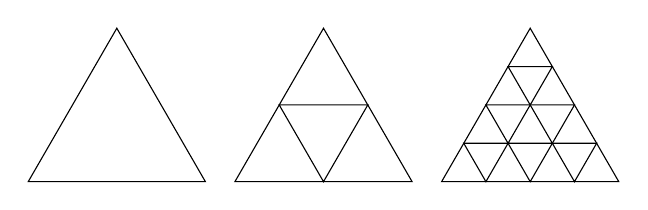
\begin{tikzpicture}[every/.style={line join=miter}, scale=0.75]
      \draw (0,0) -- ++(60:3) -- +(-60:3) -- cycle;

      \draw (3.5, 0) -- ++(60:3) -- +(-60:3) -- cycle;
      \draw ($(3.5, 0) + (60:1.5)$) -- ++(-60:1.5) -- +(60:1.5) -- cycle;

      \draw (7, 0) -- ++(60:3) -- +(-60:3) -- cycle;
      \draw ($(7, 0) + (60:1.5)$) -- ++(-60:1.5) -- +(60:1.5) -- cycle;
      \draw ($(7, 0) + (60:0.75)$) -- ++(-60:0.75) -- +(60:0.75) -- cycle;
      \draw ($(7, 0) + (60:0.75) + (1.5, 0)$) -- ++(-60:0.75) -- +(60:0.75) -- cycle;
      \draw ($(7, 0) + (60:2.25)$) -- ++(-60:0.75) -- +(60:0.75) -- cycle;
      \draw ($(7, 0) + (60:1.5) + (-60:0.75)$) -- ++(60:0.75) -- +(-60:0.75) -- cycle;
    \end{tikzpicture}
    \end{center}
  \end{block}
  \begin{block}<3 | only@3>{Grid transfer}
    \begin{itemize}
    \item Easy for nested spaces
    \item Residual restriction, $\mathcal{R}$, via embedding (fine basis
      spans coarse, so write each $\phi_c = \sum_i \alpha_i
      (\phi_f)_i$)
    \item Prolongation, $\mathcal{P}$ can be the transpose
    \item State restriction, $\mathbb{R}$, generally injection (drop
      fine dofs)
    \end{itemize}
  \end{block}
  \begin{block}<4 | only@4>{Coarse grid operators}
    \begin{itemize}
    \item Rediscretize from UFL for problem
    \item Alternative is variational (Galerkin) operator $A_c =
      \mathcal{R} A_f \mathcal{P}$
    \item Latter can be more robust in face of discontinuities,
      variable coefficients
    \end{itemize}
  \end{block}
  \begin{block}<5 | only@5>{MG cycle infrastructure}
    \begin{itemize}
    \item Firedrake is already heavily PETSc-reliant
    \item PETSc provides configurable MG \verb|-pc_type mg| and FAS
      \verb|-snes_type fas| infrastructure, so we just use that
    \item Callbacks for assembly via shell \verb|DM| (for automagic)
    \item Also means we can use full suite of PETSc solvers as smoothers
    \end{itemize}
  \end{block}
\end{frame}

\begin{frame}
  \frametitle{Mesh hierarchies}
  \begin{itemize}[<+->]
  \item Regular nested refinement makes things easy (good place to
    start)
  \item Can do coarsening, but this may affect convergence properties
    \begin{itemize}
    \item Peter, Matt and Ridg show how do this for node-nested
      coarsening [SISC 35:173 (2013)]
    \item Matt and Gerard working on unnested coarsening: will this
      work?
    \end{itemize}
  \end{itemize}
\end{frame}
\begin{frame}[fragile]
  \frametitle{Glue}
  \begin{columns}
    \begin{column}{0.5\textwidth}
      \begin{itemize}
      \item PETSc uses \verb|DM| object to give solvers information
      \item So build \verb|DMShell| that calls back to Firedrake for
        grid transfer and operator/residual evaluation
      \item Also needed for some matrix formats for fieldsplit PCs
      \end{itemize}
    \end{column}
    \begin{column}{0.5\textwidth}
      \centering
      \includegraphics[width=\textwidth]{06-29-FEniCS-multigrid.figures/glue.pdf}
    \end{column}
  \end{columns}
\end{frame}

\begin{frame}[fragile]
  \frametitle{Grid transfers}
  \begin{itemize}
  \item Kernel to perform transfers does dual basis evaluation (to
    obtain weights)
  \item Actual transfer is then just a walk over the mesh
  \item Matrix-free for now, for low order assembled $\mathcal{R}$ and
    $\mathcal{P}$ likely better
  \end{itemize}
  \begin{block}{Prolongation}
\begin{minted}{python}
def prolong(coarse, fine):
    op2.par_loop(prolong_kernel, coarse.cells(),
                 fine(op2.WRITE, c2f_dof_map),
                 coarse(op2.READ, cell_dof_map))
\end{minted}
  \end{block}
\end{frame}

\begin{frame}[fragile]
  \frametitle{Rediscretising}
  \begin{itemize}
  \item Use UFL \verb|MultiFunction| transformer to visit form and
    replace \verb|Coefficients/Arguments| with coarser equivalent
  \item Normal calls to \verb|assemble| then work transparently
  \item Question: python-level forms contain mesh-specific data, is
    there a clean way to separate so I can use the same form on
    different levels and feed new data to it?
  \end{itemize}
\end{frame}

\begin{frame}[fragile]
  \frametitle{API}
By no means set in stone

  \begin{columns}
    \begin{column}{0.5\textwidth}
      \begin{block}{What I would like}
\begin{minted}[fontsize=\scriptsize]{python}
from firedrake import *
mesh = ...
# This could come from 
# some other refinement
hierarchy = MeshHierarchy(mesh, ...)
# Select finest mesh
fine_mesh = hierarchy[-1]
V = FunctionSpace(fine_mesh, ...)
u = Function(V)
v = TestFunction(V)
F = residual(u, v)
solve(F == 0, u, {"pc_type": "mg"})
\end{minted}
      \end{block}
    \end{column}
    \begin{column}{0.5\textwidth}
      \begin{block}<2->{What I have}
\begin{minted}[fontsize=\scriptsize]{python}
from firedrake import *
mesh = ...
hierarchy = MeshHierarchy(mesh, ...)
V = FunctionSpaceHierarchy(...)
u = FunctionHierarchy(...)
# Select finest level objects
u, V = u[-1], V[-1]
v = TestFunction(V)
F = residual(u, v)
problem = NLVP(F, u, ...)
solver = NLVSHierarchy(problem, 
              {"pc_type": "mg"})
solver.solve()
\end{minted}
      \end{block}
    \end{column}
  \end{columns}
\end{frame}

\begin{frame}[fragile]
  \frametitle{Lower level API}
  \begin{itemize}
  \item Allow users to do things by hand
  \end{itemize}
  \begin{block}{Grid transfers}
Currently matrix-free only

\begin{minted}[fontsize=\scriptsize]{python}
def prolong(coarse, fine)
def restrict(fine, coarse)
# state restriction
def inject(fine, coarse)
\end{minted}
  \end{block}

  \begin{block}{Hierarchy customisation}
    \begin{itemize}
    \item Default is to just coarsen problem and rediscretise
    \item Can instead provide list of problems
    \end{itemize}
\begin{minted}[fontsize=\scriptsize]{python}
# two-level solver
solver = NLVSHierarchy([coarse_prob,
                        fine_prob], ...)
\end{minted}
  \end{block}
\end{frame}
\begin{frame}
  \frametitle{Solver configuration}
  \begin{itemize}
  \item Control of solvers via PETSc options
  \item I'm disinclined to try and bolt something on top (even if it
    gets hairy fast!)
  \item Passing information via DMs means the composability is already
    there (e.g.~Newton preconditioned with FAS)
  \end{itemize}
\end{frame}

% \begin{frame}
%   \frametitle{An example}
%   \begin{align*}
%     -\nabla \cdot (\epsilon^2 + \frac{1}{2}|\nabla u|^2)\nabla u &= 1
%     \quad \text{in $\Omega = [-1, 1]^2$}, \\
%     u &= 0 \quad \text{on $\partial \Omega$},\\
%     u_0 &= 0.
%   \end{align*}
%   \begin{columns}
%     \begin{column}{0.75\textwidth}
%       \includegraphics[height=0.5\textheight]{06-29-FEniCS-multigrid.figures/convergence}
%     \end{column}
%     \begin{column}{0.4\textwidth}
%       6 levels, P1 elements
%     \end{column}
%   \end{columns}
% \end{frame}

\begin{frame}
  \frametitle{Summary}
  \begin{itemize}
  \item Mostly, everything Just Works
  \item Interface could do with some polishing (open to suggestions)
  \item Complicated things require more work (there is no silver
    bullet)
  \item Straightforward to build and experiment with multilevel
    solvers
  \end{itemize}
\end{frame}

\begin{frame}
  \frametitle{On the wishlist}
  \begin{itemize}
  \item MG inside fieldsplit blocks (need to provide operator and
    hierarchy for just that block)
  \item Galerkin coarse operators (matrix-free grid transfer precludes
    this for now)
  \item Better support for nonlinear smoothers (NGS and NASM in
    particular)
  \item Matrix free (need operator diagonals)
  \item Hierarchies from coarsened meshes (work ongoing in PETSc?)
  \item Semi-coarsening (for extruded meshes)?
  \end{itemize}
\end{frame}

\begin{frame}
  \frametitle{Some pointers}
  Mark Adams is giving two multigrid talks \emph{tomorrow} 3pm--5pm in
  the Grantham boardroom.

  \begin{thebibliography}{99}
  \bibitem[Brandt, 1984]{Brandt:1984} A.~Brandt, \emph{The Multigrid
      Guide} (1984).  (Somewhat polemical)
  \bibitem[Yavneh, 2006]{Yavneh:2006} I.~Yavneh and G.~Dardyk, \emph{A
      Multilevel nonlinear method} SISC 28:24-46 (2006).  (Some
    analysis of convergence of nonlinear MG)
  \bibitem[Diskin, 2005]{Diskin:2005} B.~Diskin, J.~L.~Thomas and
    R.~E.~Mineck, \emph{On quantitative analysis methods for multigrid
      solutions}  SISC 27:108-129 (2005).  (Good guide to debugging
    convergence of linear multigrid)
  \bibitem[John, 2002]{John:2002} V.~John, P.~Knobloch, G.~Matthies
    and L.~Tobiska, \emph{Non-nested multi-level solvers for finite
      element discretisations of mixed problems} Computing 68:313-341
    (2002).  (Projections for non-conforming elements)
  \end{thebibliography}
\end{frame}
\end{document}
